\documentclass[tikz,border=5pt]{standalone}
\usepackage[utf8]{inputenc}
\usepackage[T1]{fontenc}
\usepackage{lmodern,amsmath,amssymb}
\usepackage[american]{circuitikz}
\usepackage{pgfplots}
\pgfplotsset{compat=1.18}
\usetikzlibrary{circuits.logic.US,positioning,calc,arrows.meta,patterns,shapes.geometric}
\definecolor{Primary}{HTML}{1F77B4}
\begin{document}
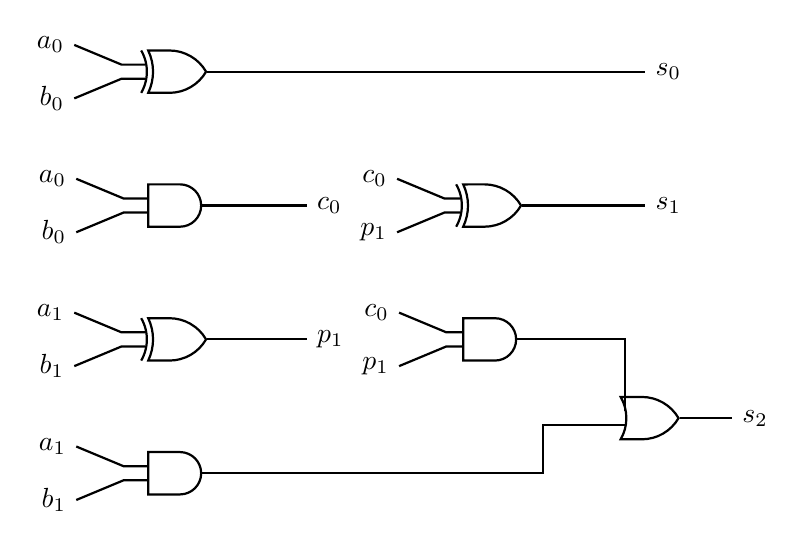
\begin{tikzpicture}[circuit logic US,thick]
\node[xor gate US,draw,logic gate inputs=nn](x0)at(1,4){};
\node[and gate US,draw,logic gate inputs=nn](c0)at(1,2.3){};
\node[xor gate US,draw,logic gate inputs=nn](p1)at(1,.6){};
\node[and gate US,draw,logic gate inputs=nn](g1)at(1,-1.1){};
\foreach \n/\a/\b in {x0/a_0/b_0,c0/a_0/b_0,p1/a_1/b_1,g1/a_1/b_1}{\draw (\n.input 1)--++(-.3,0)--++(-.6,.25)node[left]{$\a$};\draw (\n.input 2)--++(-.3,0)--++(-.6,-.25)node[left]{$\b$};}
\draw(x0.output)--(7,4)node[right]{$s_0$};\draw(c0.output)--(2.7,2.3)node[right]{$c_0$};\draw(p1.output)--(2.7,.6)node[right]{$p_1$};
\node[xor gate US,draw,logic gate inputs=nn](x1)at(5,2.3){};\draw(x1.input 1)--++(-.2,0)--++(-.6,.25)node[left]{$c_0$};\draw(x1.input 2)--++(-.2,0)--++(-.6,-.25)node[left]{$p_1$};\draw(x1.output)--(7,2.3)node[right]{$s_1$};
\node[and gate US,draw,logic gate inputs=nn](cp)at(5,.6){};\draw(cp.input 1)--++(-.2,0)--++(-.6,.25)node[left]{$c_0$};\draw(cp.input 2)--++(-.2,0)--++(-.6,-.25)node[left]{$p_1$};
\node[or gate US,draw,logic gate inputs=nn](s2)at(7,-.4){};\draw(cp.output)-|(s2.input 1);\draw(g1.output)--(5.7,-1.1)|-(s2.input 2);\draw(s2.output)--(8.1,-.4)node[right]{$s_2$};
\end{tikzpicture}
\end{document}
